\documentclass[a4 paper]{article}
\usepackage[inner=2.0cm,outer=2.0cm,top=2.5cm,bottom=2.5cm]{geometry}
\DeclareMathAlphabet{\pazocal}{OMS}{zplm}{m}{n}
\usepackage[utf8]{inputenc}
\usepackage{amsmath}
\usepackage{graphicx}
\graphicspath{{./Problem6/}}
\usepackage{mathptmx}
\usepackage{amsthm}
\usepackage{amsfonts}
\DeclareMathOperator*{\argmax}{arg\,max}

\begin{document}
	\begin{center}
  	\framebox{
    	\vbox{
      	\vspace{2mm}
        \hbox to 6.28in {{\bf CS 6140:  Machine Learning \hfill {\small Samuel Steiner steiner.s@husky.neu.edu}}}
        \vspace{5 mm}
        \hbox to 6.28in { {\Large \hfill  Homework Assignment \#1 \hfill}}
        \vspace{5 mm}
        \hbox to 6.28in {$\mathit{Assigned: 01/29/2021}$ \hfill \emph{Due:\ 02/12/2021, 11:59pm,\ through\ Canvas}}
     }
   }
    Three problems, 130 points in total. Good luck!
    
		Prof. Predrag Radivojac, Northeastern University
	\end{center}
	
	\textbf{Problem 1.} (10 points) Let $\mathit{X}, \mathit{Y}$ and $\mathit{Z}$ be discrete random variables defined as functions on the same probability space ($\Omega, \pazocal{A}, \mathit{P}$). Prove or disprove the following expression
	\[ P(X=x \mid Y=y) = \sum_{(z \in \pazocal{Z})} P(X=x\mid Y=y, Z=z) \cdot P(Z=z \mid Y=y)\]
	where $\pazocal{Z}$ is the sample space defined by the random variable $Z$
	
	\begin{proof}
	Lets say $P_y$ represents the conditional probability $P(\cdot\mid Y=y)$.
	
	Using this we can rewrite the statement as follows
	\[ P_y(X=x) = \sum_{(z \in \pazocal{Z})} P_y(X=x\mid Z=z) \cdot P_y(Z=z)\]
	
	Since $z \in \pazocal{Z}$ This is by definition of the law of total probability.
	
	Which can be proven as follows:
		\begin{equation*}
			\begin{split}
				 P(X=x) & = P(X=x \cap \bigcup_{z \in \pazocal{Z}} Z=z) \mathrm{\ Where} \pazocal{\ Z} \mathrm{\ is\ the\ sample\ space\ of\ Z} \\ 
				 & = P(\bigcup_{z \in \pazocal{Z}} X=x \cap Z=z) \\
		 		 & = \sum_{z \in \pazocal{Z}} P(X=x, Z=z) \\
		   	 & = \sum_{z \in \pazocal{Z}} P(X=x \mid Z=z)P(Z=z)
			\end{split}		
		\end{equation*}
	\end{proof}
	
	\textbf{Problem 2.} (15 points) Let $X$ be a random variable on $\pazocal{X} = \{a,b,c\}$ with the probability mass function  $p(x)$. Let $p(a) = 0.1, p(b) = 0.2,$ and $p(c) = 0.7$ and some function $f(x)$ be 
	\begin{equation*}
	f(x) = \begin{cases}
	10 & x=a \\
	5 & x=b \\
	\frac{10}{7} & x=c
	\end{cases}
	\end{equation*}
	\begin{enumerate}
	\item[a)] (5 points) What is $\mathbb{E}[f(X)]$?
	\begin{equation*}
	\mathbb{E}[f(X)] = f(a) * 0.1 + f(b) *0.2 + f(c) * 0.7 = 1 + 1 + 1 = 3
	\end{equation*}
	\item[b)] (5 points) What is $\mathbb{E}[1/p(X)]$? 
	\begin{equation*}
	\mathbb{E}[1/p(x)] = (1/p(a))*p(a) + (1/p(b))*p(b) + (1/p(c))*p(c) =1+1+1 = 3
	\end{equation*}
	\item[c)] (5 points) For an arbitrary finite set $\pazocal{X}$ with $n$ elements and arbitrary $p(x)$ on $\pazocal{X}$ what is $\mathbb{E}[1/p(X)]$?
	
	The value of this should always be $n$ since by definition $\mathbb{E}[K] = \sum_{k\in K}{(kp(k))}$ in this case $K$ is replaced with $1/p(X)$ which gets us $\mathbb{E}[1/p(X)] = \sum_{x \in X} 1/p(x)*p(x) = \sum_{x \in X}{1}$ which is equal to the size of $X$ or $n$.
	\end{enumerate}
	
	\textbf{Problem 3.} (15 points) A biased four sided die is rolled down and the down face is a random variable $X$ described by the following pmf.
	\begin{equation*}
	p(x) = \begin{cases} 
	x/10 & x=1,2,3,4 \\
	0 & \text{otherwise}
	\end{cases}
	\end{equation*}
	Given the random variable $X$ a biased coin is flipped and the random variable $Y$ is 1 or zero according to whether the coin shows heads or tails. The conditional pmf is 
	\begin{equation*}
		p(y \mid x) = \left(\frac{x+1}{2x}\right)^y\left(1 - \frac{x+1}{2x}\right)^{1-y}
	\end{equation*}
	Where $ y \in \{0, 1\}$.
	\begin{enumerate}
		\item[a) (5 points)] Find the expectation $\mathbb{E}[X]$ and the variance $V[X]$
		\begin{equation*}
			\begin{split}
				\mathbb{E}[X] & = 1(\frac{1}{10}) + 2(\frac{2}{10}) + 3(\frac{3}{10}) + 4(\frac{4}{10})\\
				& = 3
			\end{split}
		\end{equation*}
		\begin{equation*}
			\begin{split}
				V(X) & = \mathbb{E}[X^2] - (\mathbb{E}[X])^2  \\
				& = (1(\frac{1}{10})+4(\frac{2}{10})+9(\frac{3}{10})+16(\frac{4}{10})) - 3^2 \\
				& =  \frac{1}{10} + \frac{8}{10} + \frac{27}{10} + \frac{64}{10} - 9 \\
				& = 1
			\end{split}
		\end{equation*}
		\item[b) (5 points)] Find the conditional pmf $p(x\mid y)$
		\begin{equation*}
			\begin{split}
			p(y) & = \sum_{x\in X} p(y|x)p(x) \\
			& = \sum_{x=1}^4\left( \frac{x+1}{2x}\right)^y\left(1 - \frac{x+1}{2x} \right)^{1-y}\left(\frac{x}{10}\right)\\
			& = \frac{(2 \cdot 0^{(1 - y)} + 2^{(1 + y)} + 3^y + 3^{(1 - y)}\cdot 5^y)}{20}\\
			&\text{since } y \in \{0, 1\} \text{ we can write this simply as} \\
			& = \left(\frac{7}{10}\right)^y\left(\frac{3}{10}\right)^{1-y}	\\
			p(x \mid y) & = \frac{p(x)p(y\mid x)}{p(y)}	\\
			& = \frac{\frac{x}{10}\left(\frac{x+1}{2x}\right)^y\left(1 - \frac{x+1}{2x}\right)^{1-y}}{\left(\frac{7}{10}\right)^y\left(\frac{3}{10}\right)^{1-y}} \\ 
			& \text{Which can be written as} \\
			& = \begin{cases} \frac{\frac{x}{10}\left(\frac{x+1}{2x}\right)}{\frac{7}{10}} & y=1 \\
	 \frac{\frac{x}{10}\left(1-\frac{x+1}{2x}\right)}{\frac{3}{10}}& y=0 \\
	 0 & \text{otherwise}
	\end{cases}
			\end{split}
		\end{equation*}
		\item[c) (5 points)] Find the conditional expectation $\mathbb{E}[X \mid Y=1]$; i.e., the expectation with respect to the conditional pmf $p_{X\mid Y}(x\mid 1)$.
		\begin{equation*}				
		\begin{split}\
		\mathbb{E}[X \mid Y=1] & = \sum_{x=1}^4 x\left(\frac{\frac{x}{10}\left(\frac{x+1}{2x}\right)}{\frac{7}{10}}\right) \\
		& = \frac{20}{7}
		\end{split}
		\end{equation*}
	\end{enumerate}
	\textbf{Problem 4.} (25 points) suppose that data set $\pazocal{D} = \{1, 0, 1, 1, 1, 0, 1, 1, 1, 0\} $ is an i.i.d. sample from a Bernoulli distribution
	\begin{equation*}
	p(x \mid \alpha) = \alpha^x(1-\alpha)^{1-x} \qquad 0 < \alpha <1
	\end{equation*}
	with unknown parameter $\alpha$
	\begin{enumerate}
	\item[a) (5 points)] Calculate the log-likelihood of the data $\pazocal{D}$ when $\alpha = \frac{1}{e}$; i.e., find $\log{p(\pazocal{D} \mid \alpha = 1/e)}$. The parameter $e$ is the Euler number. Write the final expression as compactly as you can.
	\begin{equation*}	
	\begin{split}\
	 \sum_{d \in \pazocal{D}} \log{p(d \mid \alpha)} & = \sum_{d \in \pazocal{D}}\log{((1/e)^d(1-(1/e))^{1-d})} \\
	 & \text{Which maps} \\
	 & = \begin{cases}
	 \log{(1/e)} = -1 & 1 \\ 
	 \log{(1-(1/e))} \approx  -0.46 & 0
	 \end{cases} \\
	 & \text{for the data set } \pazocal{D} \\
	 & = -7 + 3(\log{(1-(1/e))}) \\
	 & = -10 + 3(\log{(e-1)})
	\end{split}	
	\end{equation*}
	\item[b (10 points)] Compute the maximum likelihood estimate of $\alpha$. Show all your work. 
	\begin{equation*}
	\begin{split}
	\hat{\alpha} & = \argmax_{\alpha}{\mathit{LL}(\alpha)}\\ 
	\mathit{LL}(\alpha)  &= \sum_{d \in \pazocal{D}} \log(((\alpha)^d(1-(\alpha))^{1-d}) \\
	& \text{with our dataset this becomes} \\
	& = 7(\log{\alpha}) + 3(\log{(1-\alpha})) \\
	& \text{now we do the first derivative and set it to 0} \\
	\frac{\delta\mathit{LL(\alpha)}}{\delta\alpha} & = \frac{7}{\alpha} + \frac{3}{\alpha -1} = 0  \\ 
	0 & = \frac{10 \alpha - 7}{(\alpha - 1)\alpha} \\
	0 & = 10\alpha - 7 \\
	7 & = 10\alpha  \\
	\frac{7}{10} & = \alpha 
	\end{split}
	\end{equation*}
	\item[c (10 points)] Suppose the prior distribution for $\alpha$ is the uniform distribution on $(0, 1)$ compute the Bayes estimator for $\alpha$. Note that $\int_0^1 v^m(1-v)^rdv = \frac{m!r!}{(m+r+1)!}$.
	\begin{equation*}
	\begin{split}
	\argmax_{\alpha} p({\alpha \mid \pazocal{D}}) & = p(\pazocal{D} \mid \alpha)p(\alpha) \\
	& = \mathit{LL}(p(\pazocal{D} \mid \alpha)p(\alpha)) \\
	& = \log(p(\pazocal{D} \mid \alpha)) + \log p(\alpha) \\
	& = \log(p(\pazocal{D} \mid \alpha)) + \log p(1) \\
	& \text{We already solved maximization of} \log{p(\pazocal{D} \mid \alpha)} \\
	0 & = 10\alpha - 7 \\
	7 & = 10\alpha  \\
	\frac{7}{10} & = \alpha 
	\end{split}
	\end{equation*}
	\end{enumerate}
	\textbf{Problem 5.} (10 points) Let $\pazocal{D} = \{X_i\}^n_{i=1} $ be an i.i.d. sample from 
	\begin{equation*}
	p(x) = \begin{cases}
	e^{-(x-\theta_0)} & x \geq \theta_0 \\
	0 & \text{otherwise}
	\end{cases}
	\end{equation*}
	Determine $\theta_{ML}$ - the maximum likelihood estimate of $\theta_0$. 
	\begin{equation*}
	\begin{split}
	\log{p(\pazocal{D} \mid \theta_0)} & = \log{\prod_{i=1}^n p(x_i \mid \theta_0)} \\
	& = \sum_{i=1}^n \log{e^{-(x-\theta_0)}} \\
	& \text{Now take the derivative} \\
	\frac{\delta}{\delta\theta_0} \sum_{i=1}^n \log{e^{-(x-\theta_0)}} & = n
	\end{split}
	\end{equation*}
	\textbf{Problem 6.} (25 Points) Understanding the curse of dimensionality. Consider the following experiment: generate $n$ data points with dimensionality $k$. Let each data point be generated using a uniform random number generator with values between 0 and 1. Now, for a given $k$, calculate
	\begin{equation*}
	r(k) = \log_{10}{\frac{d_{\text{max}}(k) - d_{\text{min}}(k)}{d_{\text{ave}}(k)}}
	\end{equation*}
	where $d_{\text{max}}(k)$ is the maximum distance between any par of points, $d_{\text{min}}(k)$ is the minimum distance between any pair of points (you cannot use identical points to obtain the minimum distance of 0), and $d_{\text{ave}}$ is the average distance between pairs of distinct points in the data set. Let $k$ take each value from $\{1,2,\ldots, 99, 100\}$. Repeat each experiment multiple times to get stable values by averaging the quantities over multiple runs for each $k$.
	\begin{enumerate}
	\item[a)] (10 points) Using Euclidean distance to compute $d_\text{max}$ and $d_\text{min}$, plot $r(k)$ as a function of $k$ for two different values of $n; n \in \{100, 1000\}$. Label and scale each axis properly to be able to make comparisons over different $n$’s. Embed your final picture(s) in the file you are submitting for this assignment.
		\begin{figure}[h]
		\centering
		\begin{minipage}{.5\textwidth}
  			\centering
  			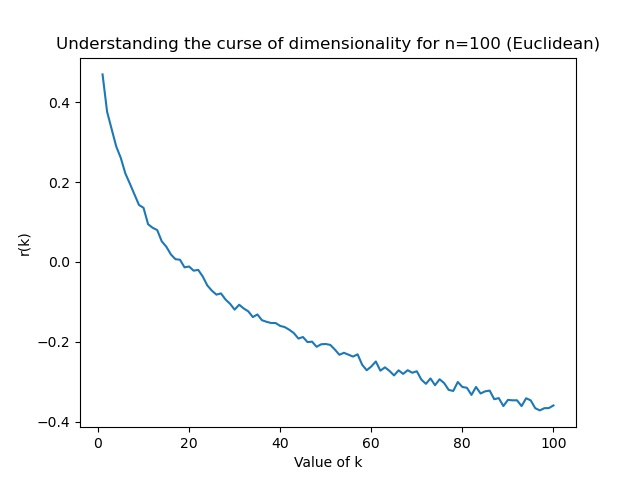
\includegraphics[width=.4\linewidth]{100_Euclidean}
  			\caption{Curse of dimensionality $n=100$}{Euclidean Distance}

		\end{minipage}%
		\begin{minipage}{.5\textwidth}
  			\centering
  			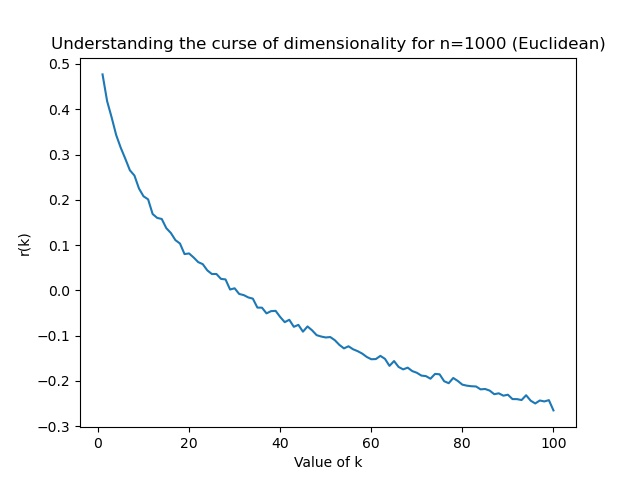
\includegraphics[width=.4\linewidth]{1000_Euclidean}
  			\caption{Curse of dimensionality $n=1000$}{Euclidean Distance}

		\end{minipage}
	\end{figure}
	\item[b)] (10 points) Replace Euclidean distance by the cosine distance, defined as $d_\text{cos}(x,y) = 1 - \cos{(x,y)}$, where $x$ and $y$ are $k$-dimensional data points and $\cos{(x,y)}$ is the cosine similarity. Then repeat the experiment from part a.
			\begin{figure}[h]
		\centering
		\begin{minipage}{.5\textwidth}
  			\centering
  			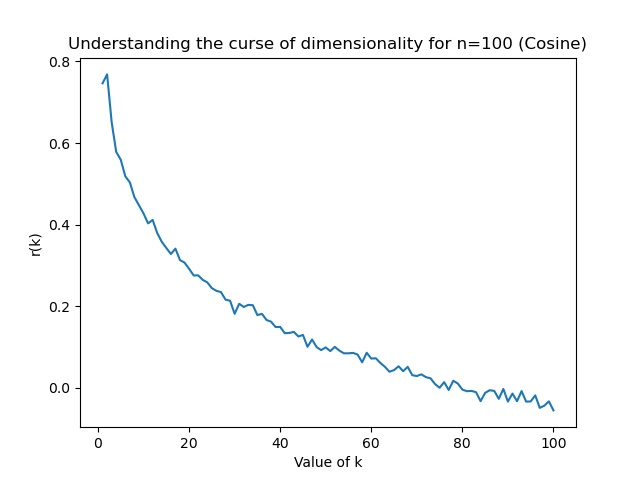
\includegraphics[width=.4\linewidth]{100_Cosine}
  			\caption{Curse of dimensionality $n=100$}{Cosine Distance}

		\end{minipage}%
		\begin{minipage}{.5\textwidth}
  			\centering
  			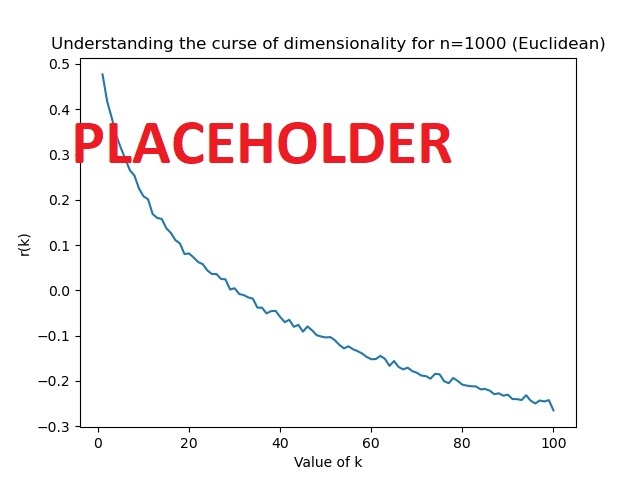
\includegraphics[width=.4\linewidth]{1000_Cosine}
  			\caption{Curse of dimensionality $n=1000$}{Cosine Distance}
		\end{minipage}
	\end{figure}		
	\item[c)] (5 points) Discuss your observations and also compare the results to your expectations before you carried out the experiments in parts a and b.
	
	My initial thoughts were that the graphs would like a normal log graph where the denominator is growing larger than the numerator that is to say the graph trends in the negative direction and 'flattens' out. This is all I really assumed when I first saw the experiment. As I predicted this is what the result was, this shows that with higher dimensionality it may be harder to find distinct differences in the data. The 1000 cosine, graphic was corrupted and I was unable to reproduce it by the time submission was necessary. 
	
	\end{enumerate}
	\textbf{Problem 7.} (30 points) Expectation-Maximization (EM) algorithm. Let $X$ be a random variable distributed according to
	\begin{equation*}
	p(x) = \alpha q(x\mid \lambda_1)+(1-\alpha)q(x \mid \lambda_0)
	\end{equation*}
	where $\alpha \in (0, 1)$ Let $q(x \mid \lambda) = \frac{\lambda}{x^{\lambda+1}}$ on the input space $[1, \inf )$ be a Pareto distribution with $\lambda > 0$. Let now $\pazocal{D} = \{x_i\}_{i=1}^n$ be a set of observations.
	\begin{enumerate}
	\item[a)] (10 points) Derive update rules of the EM algorithm to estimate, $\alpha$, $\lambda_0$, and $\lambda_1$.
	\begin{equation*}
	\begin{split}
	\theta^t &= ( \alpha^t, \lambda_0^t, \lambda_1^t) \\
	\alpha_0 &= \alpha \\  
	k & = \{0, 1\} \\
	1. \text{intialize } \alpha, \lambda_0, \text{and } \lambda_1 \text{at } t=0 \\
	2. \text{Repeat until convergence } \\ 
	\text{(a) } q_{Y_i} (k \mid x_i, \theta^t) & = \frac{\alpha_k^t q(x_i|\lambda_k^t)}{\sum_{j=0}^1 \alpha_j^t q(x_i \mid \lambda_j^t)} \text{for } \forall (i,k) \\
	\text{(b) } \alpha_k^{t+1} & = \frac{1}{n} q_{Y_i}(k \mid x_i, \theta^t) \\
	\text{(c) } \lambda_k^{t+1} & = \frac{\sum_{i=1}^n q_{Y_i}(k \mid x_i,\lambda^t)}{\sum_{i=1}^n x_i q_{Y_i}(k \mid x_i, \theta^t)} \\
	\text{(d) } t & = t + 1
	\end{split}
	\end{equation*}
	\item[b)] (20 points) Implement the learning algorithm from part a and evaluate it on 100 simulated datasets with $n$ no less than 100. Each dataset should be generated according to a distribution with fixed parameters. To assess the quality of your estimates, visualize the distribution of absolute differences between estimated and true parameters using box plots and compute the mean absolute difference. Discuss your experiments, discuss steps and calls you needed to make, and report on the quality of your algorithm.
	\end{enumerate}
\end{document}